%!TEX TS-program = xelatex
%!TEX encoding = UTF-8 Unicode

\documentclass[8pt]{article}
\usepackage[a4paper]{geometry}
\usepackage[english]{babel}
\usepackage{amssymb,amsthm,amsmath}
%\usepackage{xltxtra}
%\usepackage{stmaryrd}
\usepackage{tikz}
\usepackage{caption}
\usepackage{subcaption}
\usepackage{float}
\usepackage{graphicx}
\usepackage{listings}
\usepackage{xcolor}
\usepackage[most]{tcolorbox}
\usepackage{tabularx}
\usetikzlibrary{decorations.pathmorphing,positioning}
\usepackage[explicit]{titlesec}

\graphicspath{ {./images/} }

\definecolor{universityred}{RGB}{147,25,50}
\definecolor{complementaryb}{RGB}{25,147,122}
\definecolor{complementaryo}{RGB}{246,152,84}
\definecolor{complementaryg}{RGB}{110,147,25}

\lstset{
	extendedchars=true,
	showstringspaces=false,
	escapeinside=``,
	keywordstyle=\color{blue},
	commentstyle=\color[rgb]{0.133,0.545,0.133},
	columns=flexible,
	language=python,
	tabsize=2,
	basicstyle=\normalsize\selectfont\ttfamily,
	numbers=left,
	frame=lines,
	breaklines=true
}
\geometry{
	left=25mm,
	right=25mm,
	top=15mm,
	bottom=15mm
}
\usepackage{multicol}
\setlength{\columnsep}{1cm}

\counterwithin{figure}{section}





%%%%%%NOUVELLES COMMANDES
\newcommand{\rules}[1]{\textcolor{universityred}{#1}}
\newcommand{\problem}[1]{\section{#1}}
\newcommand{\psettings}[3]{
    \begin{tcolorbox}[colback=pink!25!white,colframe=black!25]
    \begin{center}
        \begin{tabularx}{0.9\textwidth} { 
            || >{\centering\arraybackslash}X 
            | >{\centering\arraybackslash}X 
            | >{\centering\arraybackslash}X || }
            \hline
            Problem ID & Judges & Time Limit\\
            \hline
            #1 &  #2 & #3\\
            \hline
        \end{tabularx}
    \end{center}
    \end{tcolorbox}
}
\newcommand{\ppart}[1]{\leavevmode \newline \noindent\textbf{\LARGE \textcolor{universityred}{#1}}\newline} %%%%PROBLEM PARTS
\newcommand{\psubpart}[1]{\leavevmode \newline \noindent\textbf{\Large \textcolor{universityred}{#1}}\newline} %%%%PROBLEM SUBPARTS
\newcommand{\bO}[1]{\ensuremath{\mathcal{O}(#1)}}

\newcommand{\inout}[1]{
    \begin{tcolorbox}[sharp corners,colback=white,colframe=gray]
        \begin{verbatim}
            #1
        \end{verbatim}
    \end{tcolorbox}
}

%%%%%%FIN NOUVELLES COMMANDES



\titleformat{\section}[hang]{\Large\bfseries\sffamily}%
{\rlap{\color{universityred}\rule[-6pt]{\textwidth}{1.2pt}}\colorbox{universityred}{%
           \raisebox{0pt}[13pt][3pt]{ \makebox[100pt]{% height, width
                \fontfamily{phv}\selectfont\color{white}{\thesection}}
            }}}%
{15pt}%
{ \color{universityred}PROBLEM : #1
%
}
\titlespacing*{\section}{0pt}{3mm}{5mm}



\begin{document}






%%%%%%PAGE DE COUVERTURE
    \begin{titlepage}
            \begin{center}
        \vspace*{1cm}
        
        \Huge
        
        \textbf{Internal Selection for ICPC-SWERC}
        
        \vspace*{0.5cm}
        
        
        \textit{\Large Paris, day month year}
        
        
        
        
        
        \vspace*{2.5cm}
        
        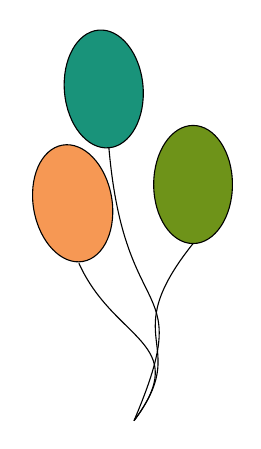
\begin{tikzpicture}
            \filldraw[fill=complementaryg, draw=black](0,2) ellipse (.5cm and .75cm);
            \draw (-0.75,-1) .. controls (0,0) and (-1.,0) .. (0,1.25);
            \draw (-0.75,-1) .. controls (0,0) and (-1.,0) .. (-1.45,1);
            \draw (-0.75,-1) .. controls (0.1,1) and (-1.,0) .. (-1.1,3);
            \draw[rotate around={10:(0,0)},fill=complementaryo, draw=black] (-1.2,2) ellipse (.5cm and .75cm);
            \draw[rotate around={5:(0,0)},fill=complementaryb, draw=black] (-0.85,3.3) ellipse (.5cm and .75cm);
        \end{tikzpicture}
        
        
\includegraphics[scale=0.025]{./titlepage/images/cover_image.png}
        
        \vspace*{2.5cm}
        
        
        
        \begin{tcolorbox}[enhanced,attach boxed title to top center={yshift=-2mm,yshifttext=-4mm},
        colback=pink!25!white,colframe=black!25,colbacktitle=universityred,
        title= \strut Judges and problem settlers,fonttitle=\Large \bfseries,
        boxed title style={size=small,colframe=red!50!black, top = 3mm, bottom = 2mm, left = 7mm, right = 7mm} ]
            \large
            \begin{multicols}{3}
                    \begin{itemize}
                        \item Judge 1, \textit{Chief judge}
                        \item Judge 2
                        \item Judge 3
                        \item Judge 4
                        \item Judge 5
                        \item Judge 6
                    \end{itemize}
            \end{multicols}
        \end{tcolorbox}
        
        
        
        \vfill
        
        \large
        \textbf{Université Paris Cité}\\
        UFR de Mathématiques-Informatique
        2022-2023\\
    \end{center}
    
    
    \small Template by Hugo Demaret
    \hfill 
    2022
    \end{titlepage}
%%%%%%FIN PAGE DE COUVERTURE


%%%%%%PAGE DE SEPARATION
    \newpage

\vspace*{\fill}

\begin{center}
    
    
    
    \textit{\Large This page is left intentionally blank.}
    
    \vspace*{2.5cm}
    
    
\begin{tikzpicture}
            \filldraw[fill=complementaryg, draw=black](0,2) ellipse (.5cm and .75cm);
            \draw (0,-1) .. controls (0,0) and (-1.,0) .. (0,1.25);
    \end{tikzpicture}
        
\end{center}

\vspace*{\fill}

\newpage
%%%%%%PAGE DE SEPARATION
    


%%%%%%REGLES DU CONCOURS
    \begin{center}
    \Huge \textcolor{universityred}{Rules}
\end{center}

\begin{itemize}
    \item \rules{Règles (je suppose) similaires à celles du swerc au maximum ?}
\end{itemize}
%%%%%%FIN REGLE DU CONCOURS

%%%%%%PAGE DE SEPARATION
    \newpage

\vspace*{\fill}

\begin{center}
    
    
    
    \textit{\Large This page is left intentionally blank.}
    
    \vspace*{2.5cm}
    
    
\begin{tikzpicture}
            \filldraw[fill=complementaryg, draw=black](0,2) ellipse (.5cm and .75cm);
            \draw (0,-1) .. controls (0,0) and (-1.,0) .. (0,1.25);
    \end{tikzpicture}
        
\end{center}

\vspace*{\fill}

\newpage
%%%%%%PAGE DE SEPARATION

%%%%%%PROBLEME 1
    \problem{TITLE}
\psettings{2022-}{NAMES}{N.D}


\ppart{Input}
\ppart{Output}
\ppart{Limits}
\ppart{Examples}
\psubpart{Sample Input 1}
\psubpart{Sample Output 1}
\psubpart{Sample Input 2}
\psubpart{Sample Output 2}
\psubpart{Sample Input 3}
\psubpart{Sample Output 3}
%%%%%%FIN PROBLEME 1


%%%%%%PAGE DE SEPARATION
    \newpage

\vspace*{\fill}

\begin{center}
    
    
    
    \textit{\Large This page is left intentionally blank.}
    
    \vspace*{2.5cm}
    
    
\begin{tikzpicture}
            \filldraw[fill=complementaryg, draw=black](0,2) ellipse (.5cm and .75cm);
            \draw (0,-1) .. controls (0,0) and (-1.,0) .. (0,1.25);
    \end{tikzpicture}
        
\end{center}

\vspace*{\fill}

\newpage
%%%%%%PAGE DE SEPARATION


%%%%%%PROBLEME 2
    \problem{TITLE}
\psettings{2022-}{NAMES}{N.D}


\ppart{Input}
\ppart{Output}
\ppart{Limits}
\ppart{Examples}
\psubpart{Sample Input 1}
\psubpart{Sample Output 1}
\psubpart{Sample Input 2}
\psubpart{Sample Output 2}
\psubpart{Sample Input 3}
\psubpart{Sample Output 3}
%%%%%%FIN PROBLEME 2


%%%%%%PAGE DE SEPARATION
    \newpage

\vspace*{\fill}

\begin{center}
    
    
    
    \textit{\Large This page is left intentionally blank.}
    
    \vspace*{2.5cm}
    
    
\begin{tikzpicture}
            \filldraw[fill=complementaryg, draw=black](0,2) ellipse (.5cm and .75cm);
            \draw (0,-1) .. controls (0,0) and (-1.,0) .. (0,1.25);
    \end{tikzpicture}
        
\end{center}

\vspace*{\fill}

\newpage
%%%%%%PAGE DE SEPARATION

%%%%%%PROBLEME 3
    \problem{TITLE}
\psettings{2022-}{NAMES}{N.D}


\ppart{Input}
\ppart{Output}
\ppart{Limits}
\ppart{Examples}
\psubpart{Sample Input 1}
\psubpart{Sample Output 1}
\psubpart{Sample Input 2}
\psubpart{Sample Output 2}
\psubpart{Sample Input 3}
\psubpart{Sample Output 3}
%%%%%%FIN PROBLEME 3

%%%%%%PAGE DE SEPARATION
    \newpage

\vspace*{\fill}

\begin{center}
    
    
    
    \textit{\Large This page is left intentionally blank.}
    
    \vspace*{2.5cm}
    
    
\begin{tikzpicture}
            \filldraw[fill=complementaryg, draw=black](0,2) ellipse (.5cm and .75cm);
            \draw (0,-1) .. controls (0,0) and (-1.,0) .. (0,1.25);
    \end{tikzpicture}
        
\end{center}

\vspace*{\fill}

\newpage
%%%%%%PAGE DE SEPARATION


%%%%%%PROBLEME 4
    \problem{TITLE}
\psettings{2022-}{NAMES}{N.D}


\ppart{Input}
\ppart{Output}
\ppart{Limits}
\ppart{Examples}
\psubpart{Sample Input 1}
\psubpart{Sample Output 1}
\psubpart{Sample Input 2}
\psubpart{Sample Output 2}
\psubpart{Sample Input 3}
\psubpart{Sample Output 3}
%%%%%%FIN PROBLEME 4


%%%%%%PAGE DE SEPARATION
    \newpage

\vspace*{\fill}

\begin{center}
    
    
    
    \textit{\Large This page is left intentionally blank.}
    
    \vspace*{2.5cm}
    
    
\begin{tikzpicture}
            \filldraw[fill=complementaryg, draw=black](0,2) ellipse (.5cm and .75cm);
            \draw (0,-1) .. controls (0,0) and (-1.,0) .. (0,1.25);
    \end{tikzpicture}
        
\end{center}

\vspace*{\fill}

\newpage
%%%%%%PAGE DE SEPARATION

%%%%%%PROBLEME 5
    \problem{TITLE}
\psettings{2022-}{NAMES}{N.D}


\ppart{Input}
\ppart{Output}
\ppart{Limits}
\ppart{Examples}
\psubpart{Sample Input 1}
\psubpart{Sample Output 1}
\psubpart{Sample Input 2}
\psubpart{Sample Output 2}
\psubpart{Sample Input 3}
\psubpart{Sample Output 3}
%%%%%%FIN PROBLEME 5

%%%%%%PAGE DE SEPARATION
    \newpage

\vspace*{\fill}

\begin{center}
    
    
    
    \textit{\Large This page is left intentionally blank.}
    
    \vspace*{2.5cm}
    
    
\begin{tikzpicture}
            \filldraw[fill=complementaryg, draw=black](0,2) ellipse (.5cm and .75cm);
            \draw (0,-1) .. controls (0,0) and (-1.,0) .. (0,1.25);
    \end{tikzpicture}
        
\end{center}

\vspace*{\fill}

\newpage
%%%%%%PAGE DE SEPARATION

%%%%%%PROBLEME 6
    \problem{TITLE}
\psettings{2022-}{NAMES}{N.D}


\ppart{Input}
\ppart{Output}
\ppart{Limits}
\ppart{Examples}
\psubpart{Sample Input 1}
\psubpart{Sample Output 1}
\psubpart{Sample Input 2}
\psubpart{Sample Output 2}
\psubpart{Sample Input 3}
\psubpart{Sample Output 3}
%%%%%%FIN PROBLEME 6
    
%%%%%%DERNIERE PAGE
    \newpage

\vspace*{\fill}

\begin{center}
    
    
    
    \textit{\Large This is the last page.}
    
    \vspace*{2.5cm}
    
   
        
\end{center}

\vspace*{\fill}

\newpage
%%%%%%DERNIERE PAGE FIN
    
\end{document}